\chapter{Extraction des demandes par apprentissage automatique}

\subsection{Méthode 2: classification des sommes d'argent}

\begin{figure}[!htb]
 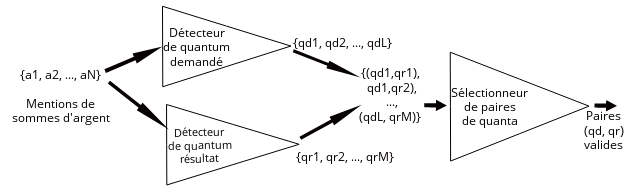
\includegraphics[scale=0.6]{extractDmd-archClassifArgent.png}
 \caption{Extraction des demandes par classification des sommes d'argent}\label{fig:quanta:classif}
\end{figure}

Les deux champs directement accessibles à partir du texte, sont les quanta demandé ($q_d$) et accordé ($q_r$). Pour les demandes à quanta, il est possible de restreindre l'extraction à ces deux variables. Le sens du résultat ($s_r$) est déduit de la valeur extraite du quantum accordé : \[s_r = \left\lbrace \begin{array}{ll}
"accepte" & \text{si } q_r > 0 \\
"rejette" & \text{sinon.} \end{array} \right.\]

L'idée est d'extraire les quanta demandés et obtenus puis de d'identifier les paires $(q_d, q_r)$ qui représentent des demandes. Le système recherche les mentions de sommes d'argent qui sont des quanta. La  détection des quanta est réalisable soit par classification individuelle des sommes d'argent, soit par inférence probabiliste du groupe de quanta. 


La performance d'une telle approche repose sur deux aspects principaux: la définition des  caractéristiques des objets à classifier, et la résolution des doublons. 

\subsubsection{Définition des caractéristiques}

La considération d'une somme d'argent comme quantum dépend de son contexte de mention et de l'histoire globale du document. Nous combinons plusieurs types de caractéristiques:
\begin{itemize}
	\item le plongement sémantique de la somme d'argent;
	\item l'agrégation pondérée du vecteur des mots qui sont dans la phrase de la somme d'argent;
    \item le plongement sémantique de la section
    \item le plongement sémantique du dispositif
    \item le plongement sémantique du document
\end{itemize}

Les caractéristiques des paires consiste en l'agrégation des vecteurs des deux sommes par concaténation, max, ou soustraction.

\subsubsection{Résolution des doublons}
Il s'agit ici des mentions de sommes d'argent à valeurs égales. Certaines sont correspondent au même quantum (par ex. quanta du MOTIFS répétés dans le DISPOSITIF). D'autres représentent des quanta différents.

 Le problème des doublons se pose déjà sur les données d'entraînement. En effet, nous devons retrouver à quelle mention de somme d'argent correspond chaque quantum du tableau des annotations manuelles. Si on annote tous les doublons comme quanta, se retrouve avec des demandes en plus. Même si on considère qu'il s'agit de la même demande, on n'en est pas sûr. On peut choisir le plus probable parmi les doublons présents.

%Résolution des doublons: classification de paires apprise sur un dataset généré à partir du comportement observé des détecteur de quanta sur le corpus d'entrainement. (a1, a2) -> (similaire, différent). UNIQUEMENT POUR DES SOMME DE VALEURS EGALES

\textcolor{red}{STATISTIQUES SUR LE TAUX DE DOUBLONS DANS LES DONNÉES ANNOTÉES}


\subsection{Méthode 3: prédiction jointe de structure}
?Apprentissage sur les documents à une seule demande pour limiter les bruits?

Pré-traitement: normalisation des sommes d'argent dans les document (par ex. 3000 euros <argent valeur="3000 euros">ARGENT\_i</argent> $i$ étant la position d'apparition de la mention)

\begin{equation}
P(D|T,A) = \sum\limits_{i=1}^{\vert D \vert} p_{\theta_1}(d_i = (a_j, a_l) | T, a_j, a_l, A) \cdot p_{\theta_2}(q_{d_i} = a_j | T, a_j, A) \cdot p_{\theta_3}(q_{r_i} = a_l | T, a_l, A)    
\end{equation}